\subsection{Montículo La Palangana}
\FloatBarrier

\begin{figure}[H]
    \centering
    \caption{Montículo La Palangana, panel de vistas}
    \label{fig:palangana-panel}
    % ----- Fila 1 -----
    \begin{subfigure}{0.48\textwidth}
        \centering
        \caption{Vista en malla (wireframe)}
        \label{fig:palangana-wire}
        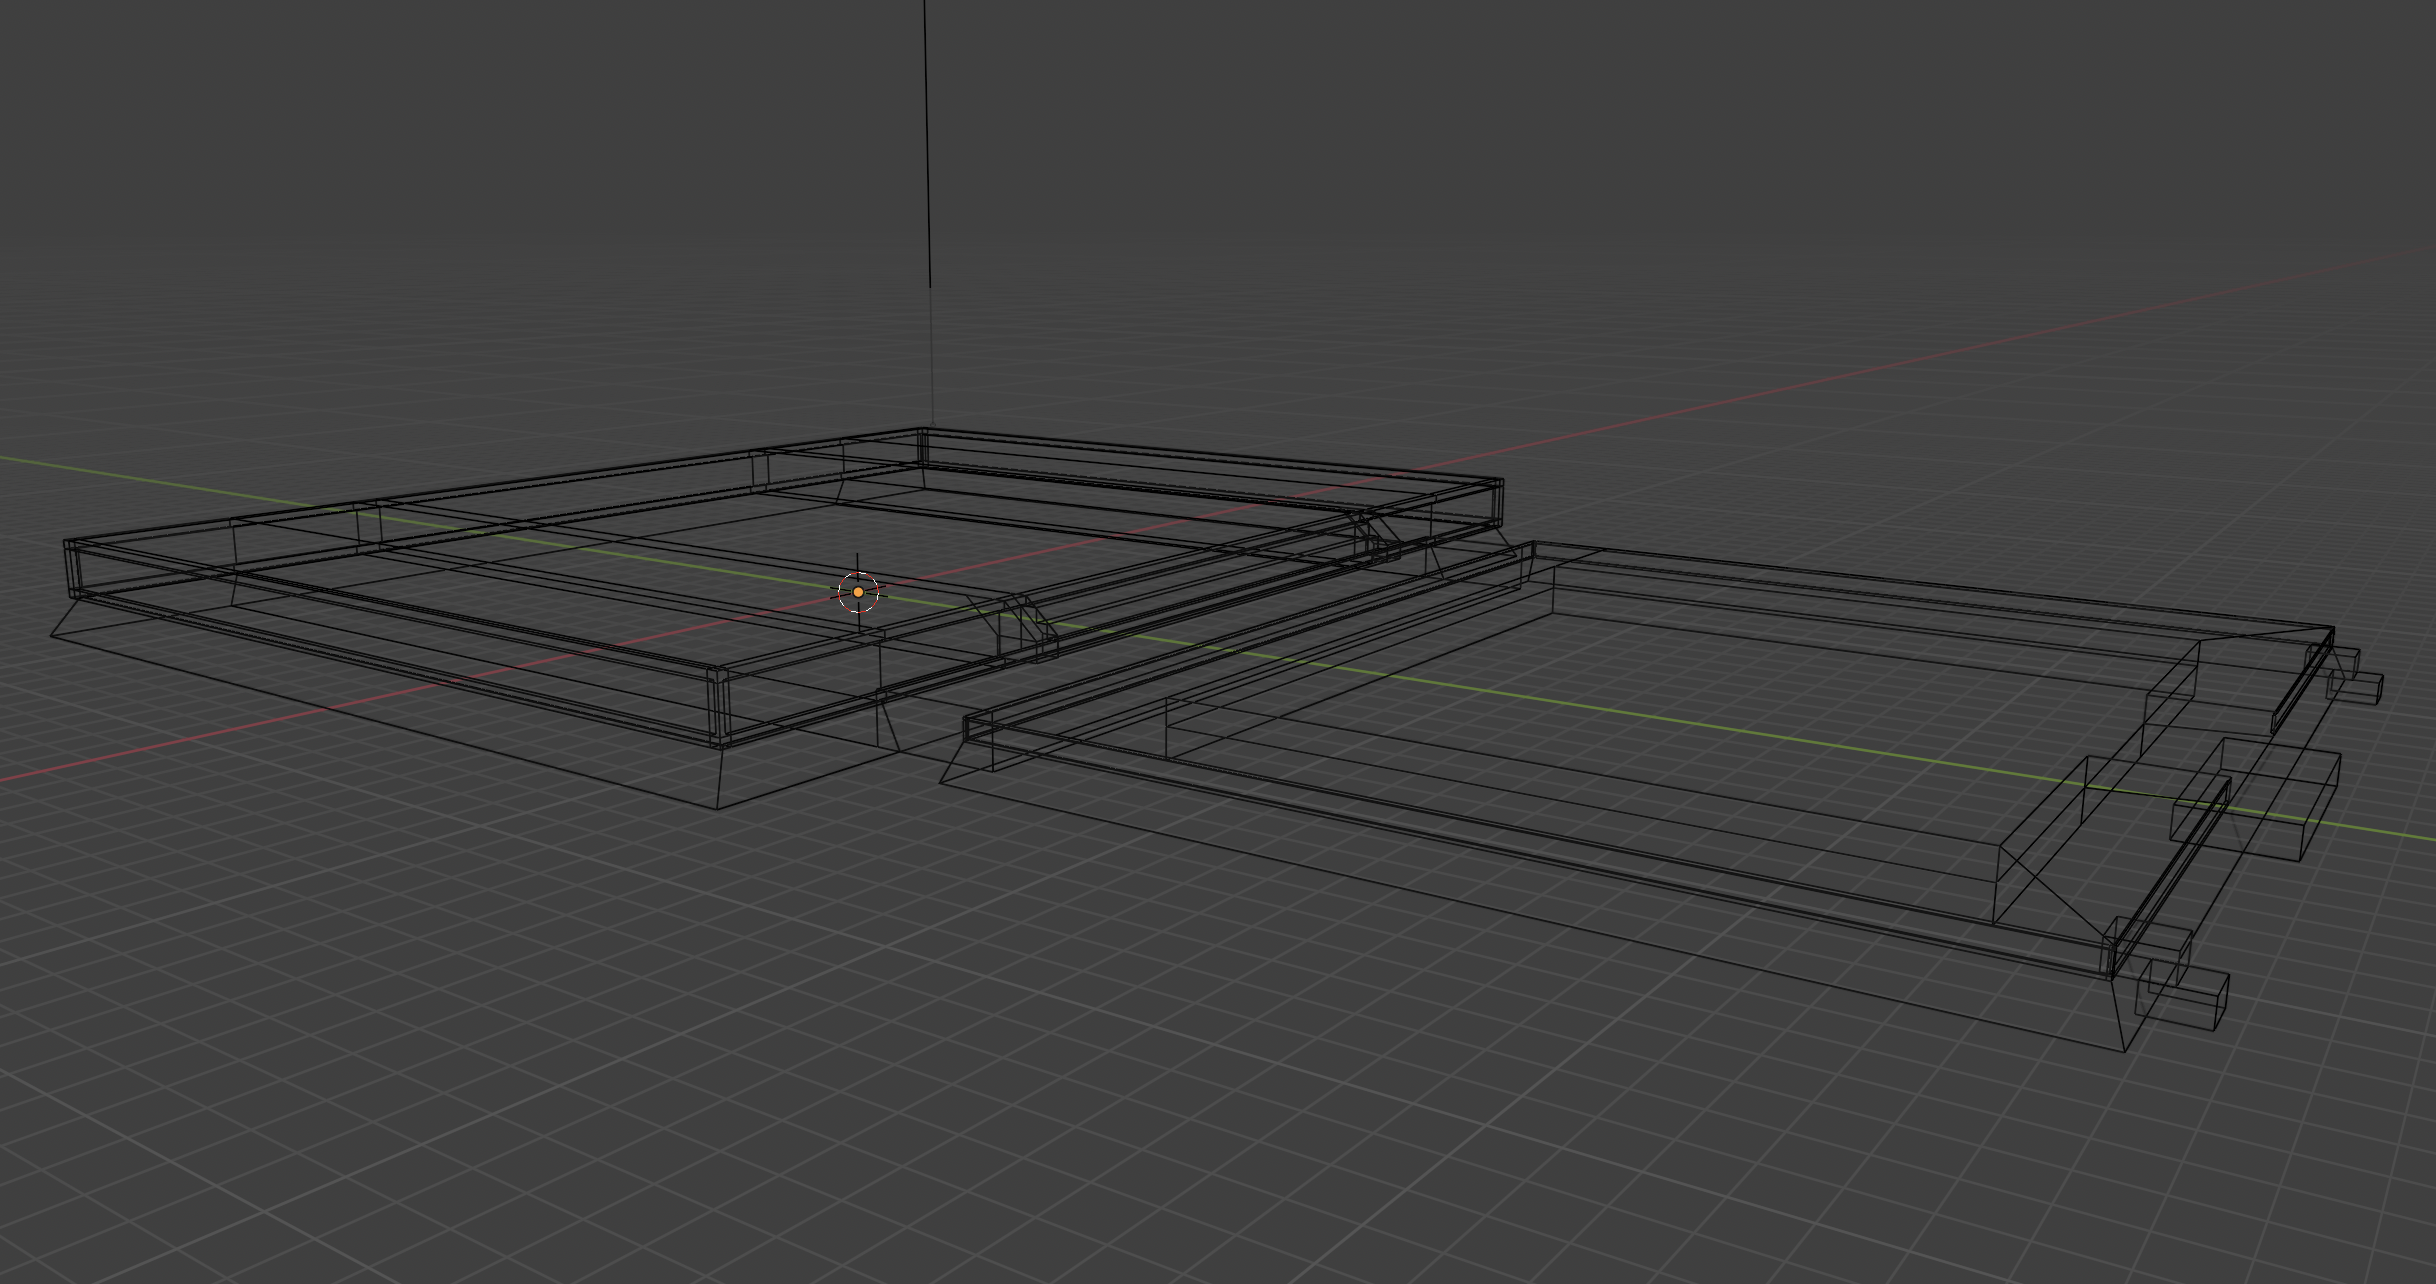
\includegraphics[width=0.85\linewidth]{resultados/figures/palangana/palangana_wireframe.png}
    \end{subfigure}\hfill
    \begin{subfigure}{0.48\textwidth}
        \centering
        \caption{Vista sólida sin texturas}
        \label{fig:palangana-solid}
        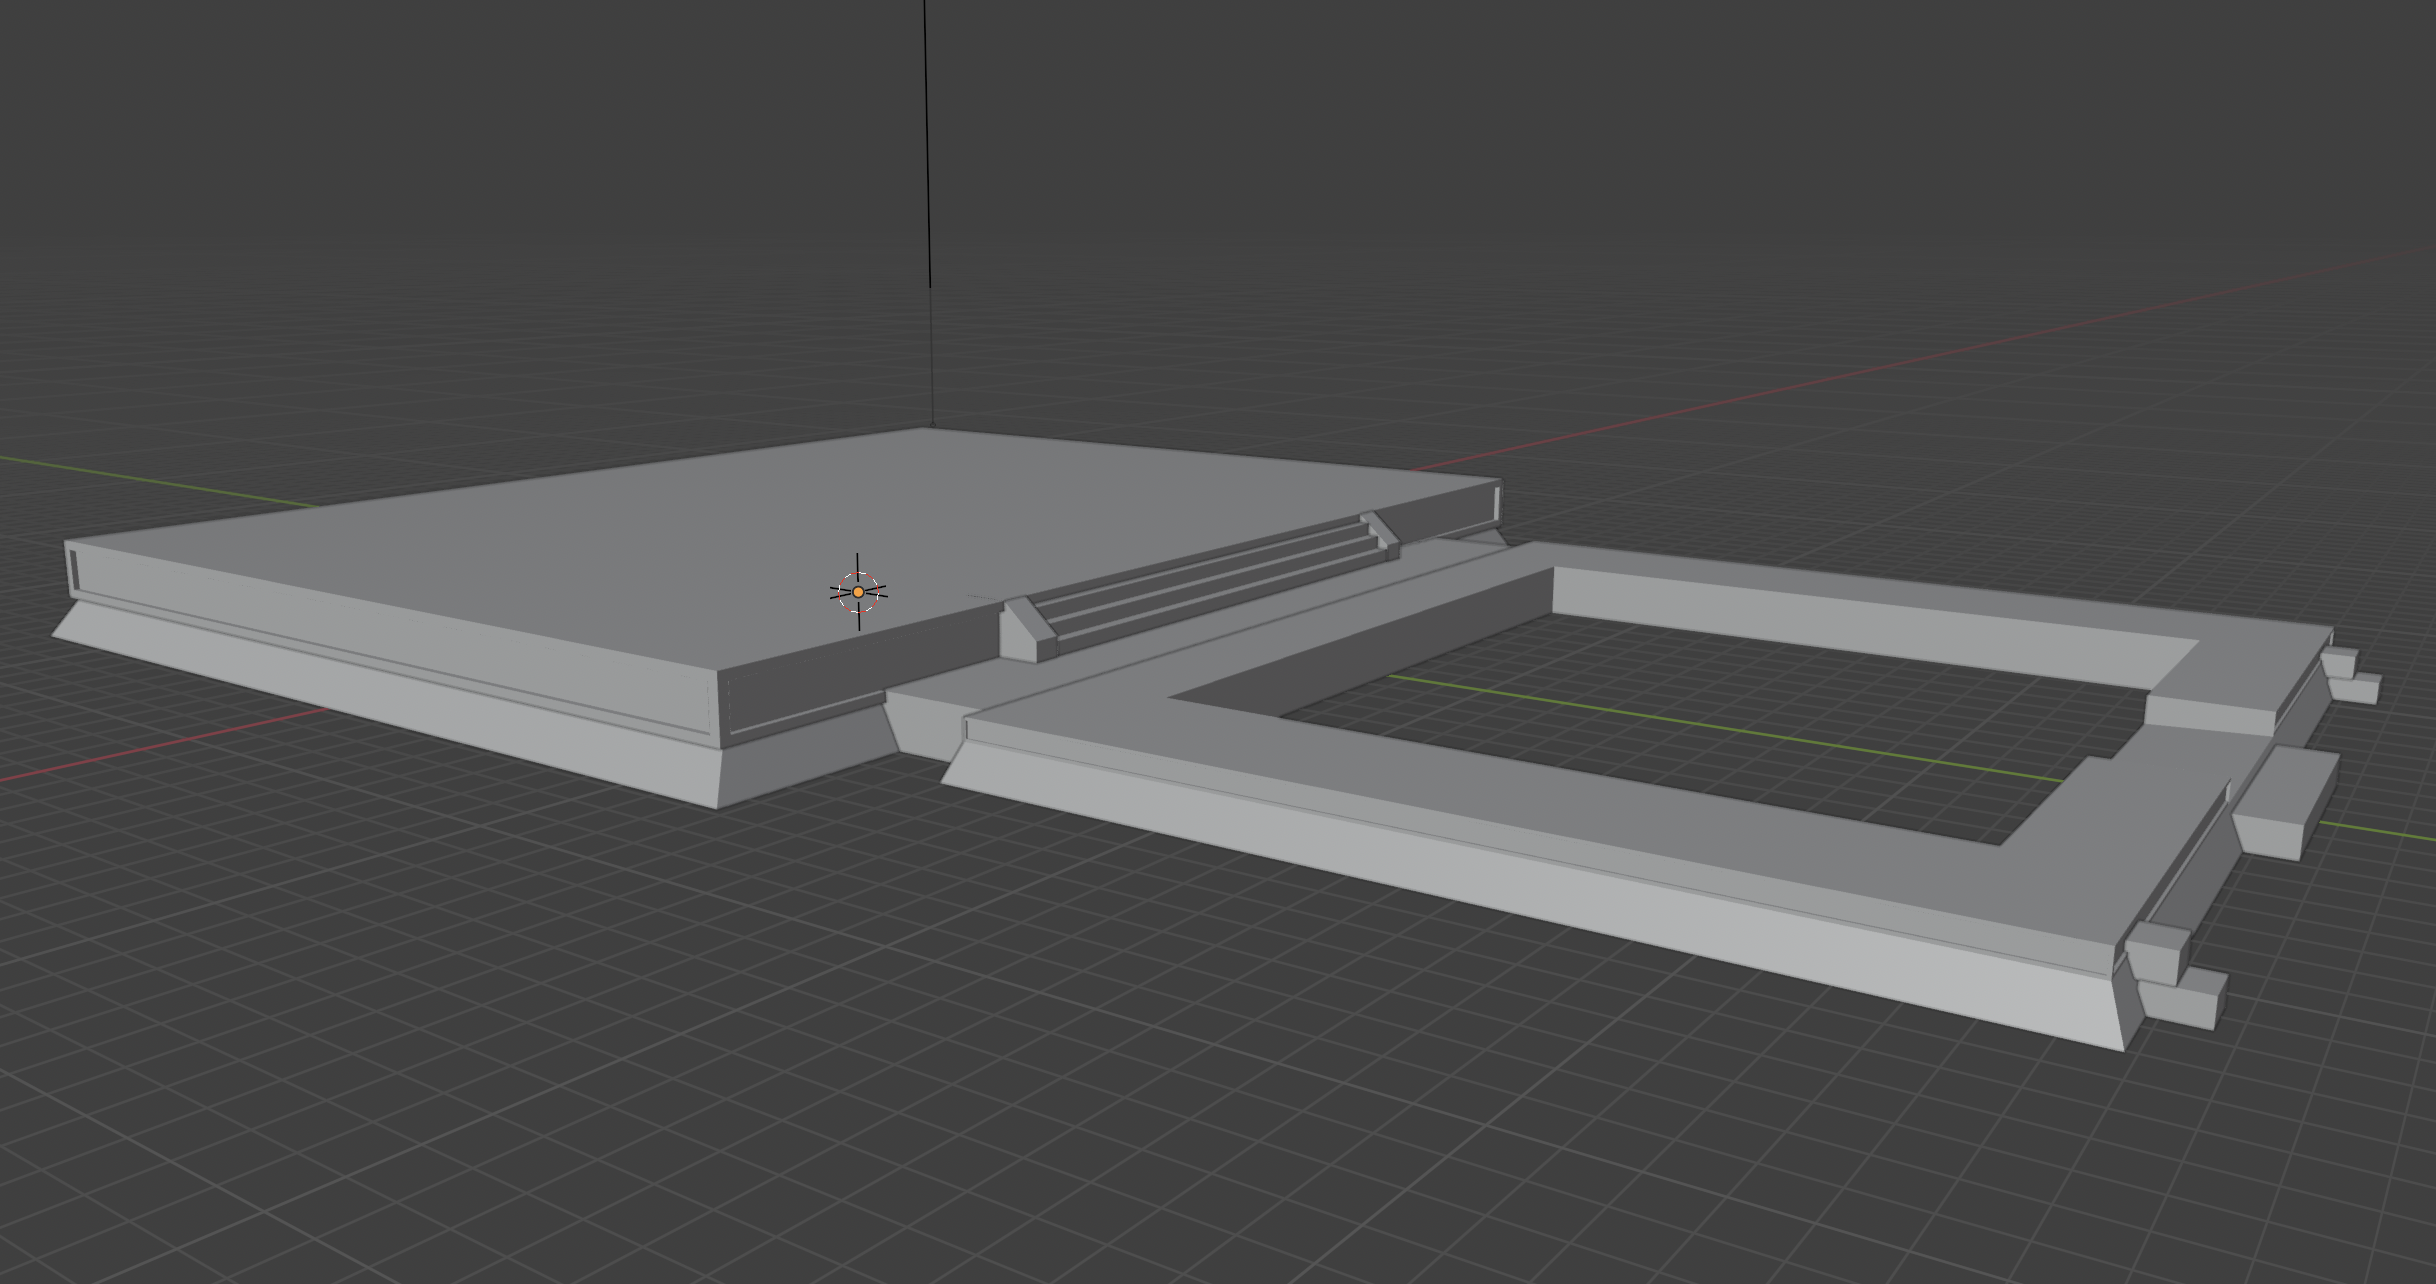
\includegraphics[width=0.85\linewidth]{resultados/figures/palangana/palangana_solid.png}
    \end{subfigure}

    \vspace{0.5em}

    % ----- Fila 2 -----
    \begin{subfigure}{0.48\textwidth}
        \centering
        \caption{Vista con materiales/texturas}
        \label{fig:palangana-textured}
        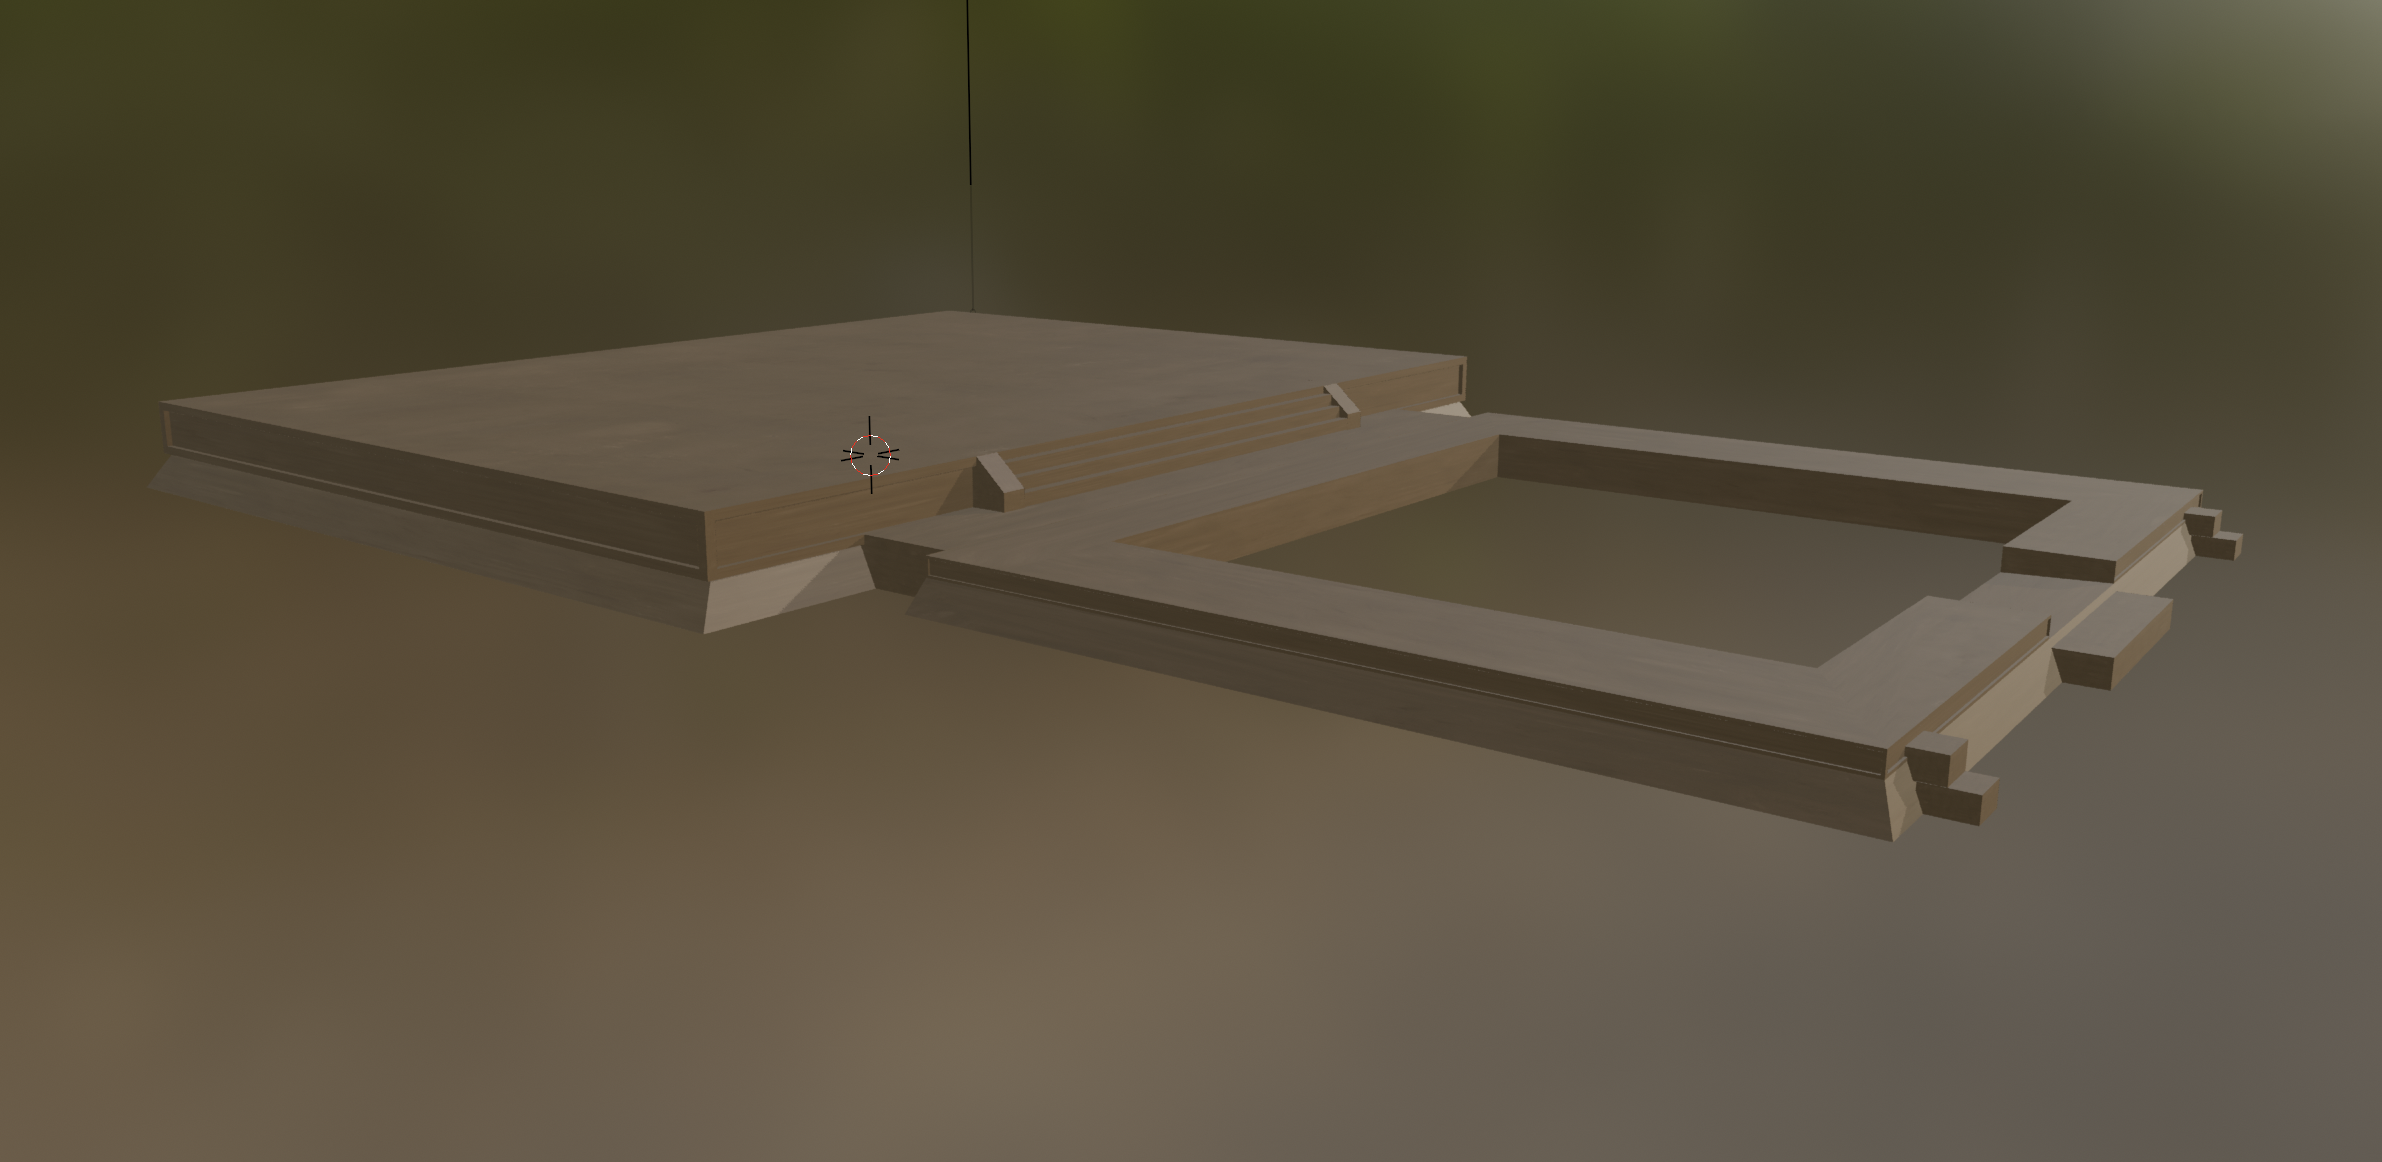
\includegraphics[width=0.85\linewidth]{resultados/figures/palangana/palangana_textured_viewport.png}
    \end{subfigure}
\end{figure}

\begin{figure}[!htbp]
    \centering
    \caption{Montículo La Palangana visualizado en la aplicación de realidad aumentada, mostrando la reconstrucción superpuesta en el entorno real del parque arqueológico}
    \label{fig:palangana-ar}
    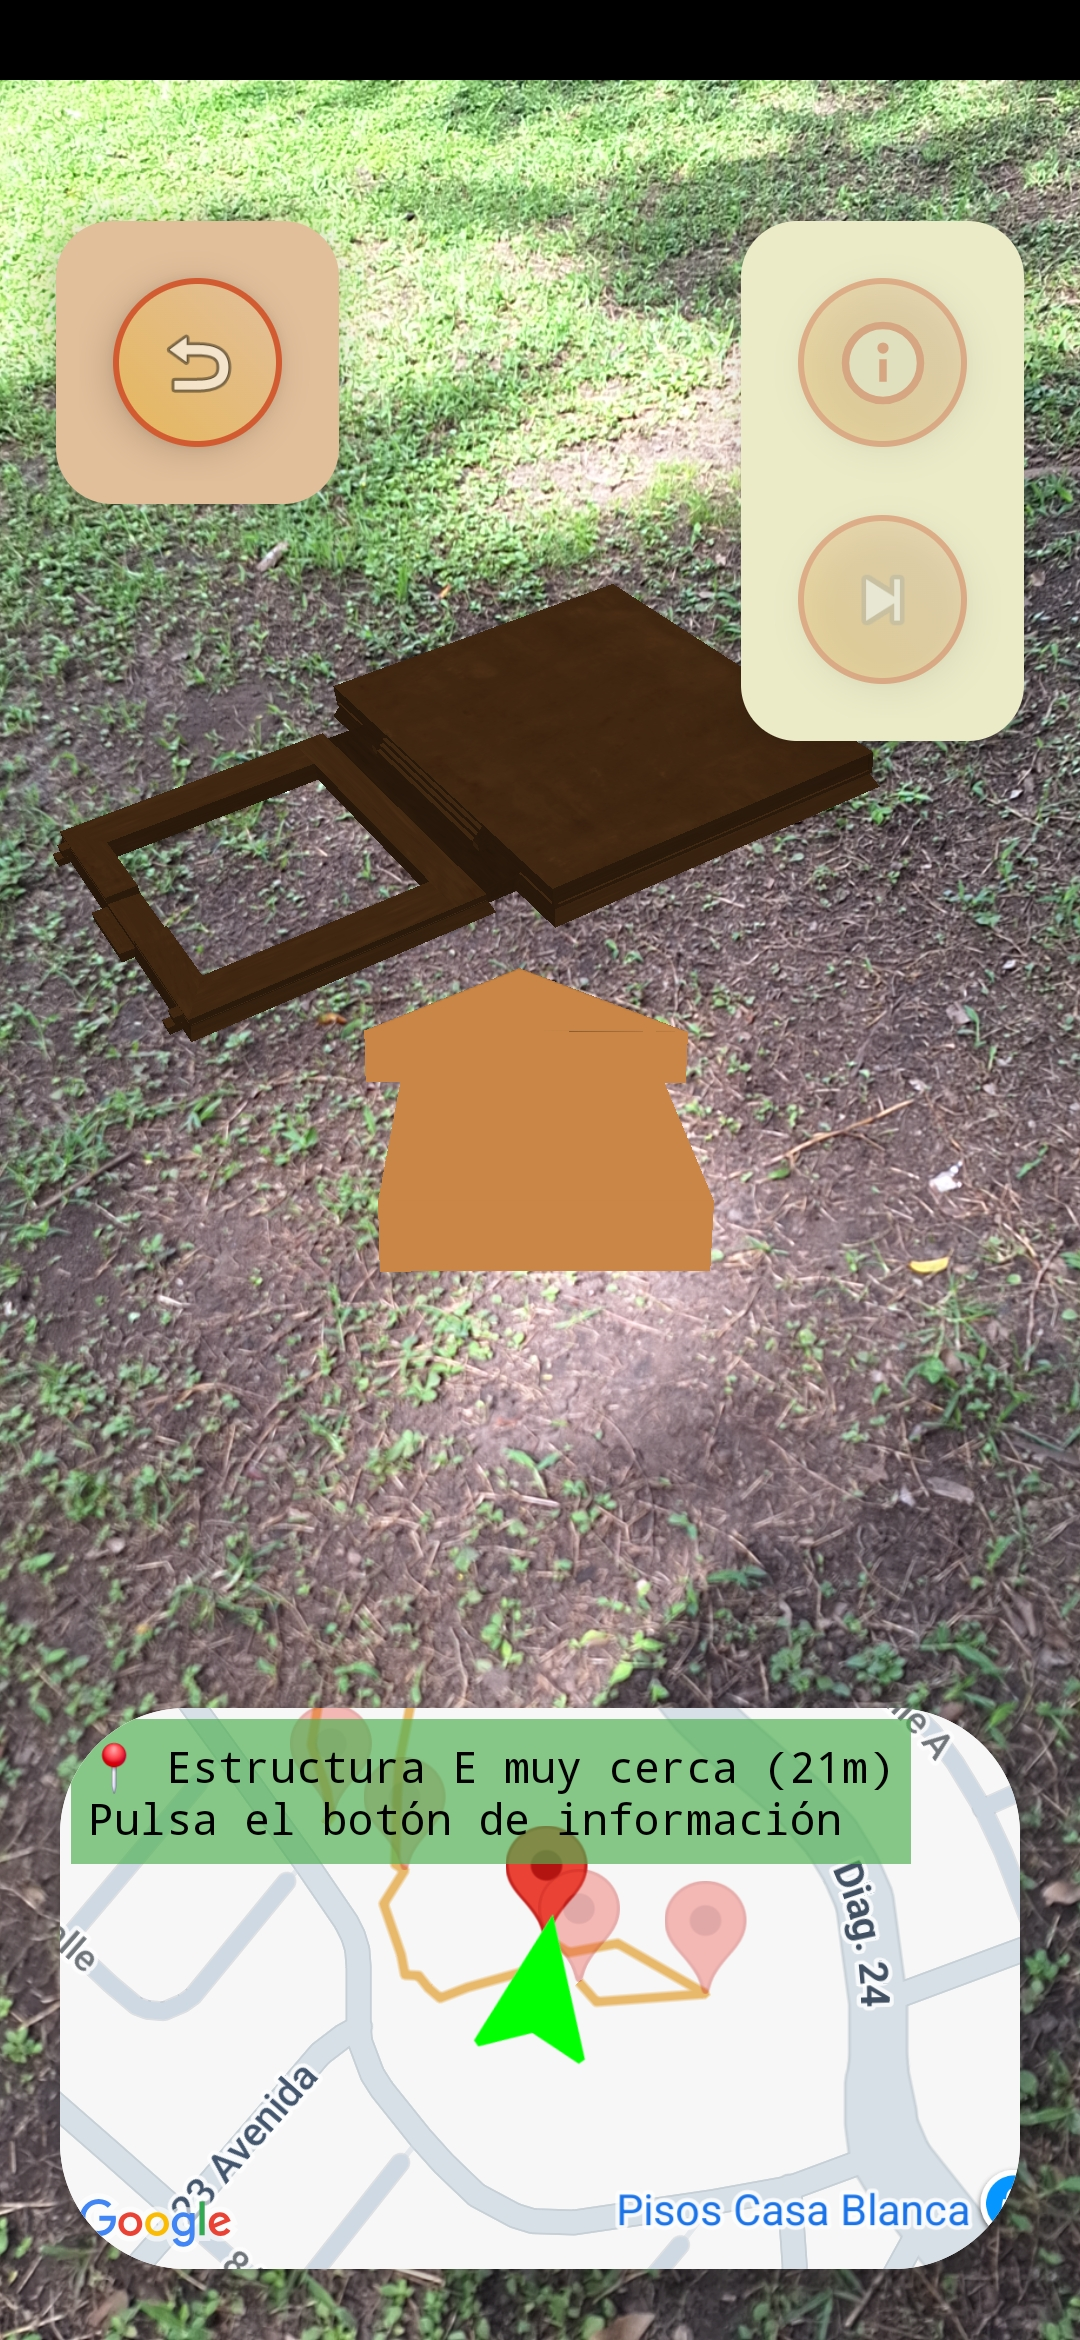
\includegraphics[width=0.28\linewidth]{resultados/figures/palangana/palangana_ar.jpg}
\end{figure}
\FloatBarrier
\clearpage